% move all configuration stuff into one file so we can focus on the content
\documentclass[aspectratio=169,hyperref={pdfpagelabels=false,colorlinks=true,linkcolor=white,urlcolor=lightblue},xcolor={table},t]{beamer}

%%%%%%%%%%%%%%%%%%%%%%%%%%%%%%%%%%%%%%%%%%%%%%%%%%%%%%%%%%%%%%%%%%%%%%%%%%%%%%%%%%
%%%%%%%%%%%%%%%%%%%%%%%%%%%%%%%%%%%%%%%%%%%%%%%%%%%%%%%%%%%%%%%%%%%%%%%%%%%%%%%%%%
% packages
\usepackage{pict2e}
\usepackage{epic}
\usepackage{amsmath,amsfonts,amssymb}
\usepackage{units}
\usepackage{fancybox}
\usepackage[absolute,overlay]{textpos} 
%\usepackage[table]{xcolor}
\usepackage{animate}
\usepackage{gensymb}
%\usepackage{graphicx}
%\usepackage{longtable}
\usepackage{multirow}
\usepackage{silence}
\usepackage{tikz}
\usepackage[backend=bibtex,style=ieee]{biblatex}
\AtEveryCitekey{\iffootnote{\tiny}{}}
%\addbibresource{include/references}



% fontsize
\let\Tiny=\tiny

%%%%%%%%%%%%%%%%%%%%%%%%%%%%%%%%%%%%%%%%%%%%%%%%%%%%%%%%%%%%%%%%%%%%%%%%%%%%%%%%%%
%%%%%%%%%%%%%%%%%%%%%%%%%%%%%%%%%%%%%%%%%%%%%%%%%%%%%%%%%%%%%%%%%%%%%%%%%%%%%%%%%%
% warnings
\pdfsuppresswarningpagegroup=1
\WarningFilter{biblatex}{Patching footnotes failed}
\WarningFilter{latexfont}{Font shape}
\WarningFilter{latexfont}{Some font shapes}
\WarningFilter{gensymb}{Not defining}


%%%%%%%%%%%%%%%%%%%%%%%%%%%%%%%%%%%%%%%%%%%%%%%%%%%%%%%%%%%%%%%%%%%%%%%%%%%%%%%%%%
%%%%%%%%%%%%%%%%%%%%%%%%%%%%%%%%%%%%%%%%%%%%%%%%%%%%%%%%%%%%%%%%%%%%%%%%%%%%%%%%%%
% theme & layout
\usetheme{Frankfurt}
\useinnertheme{rectangles}


%%%%%%%%%%%%%%%%%%%%%%%%%%%%%%%%%%%%%%%%%%%%%%%%%%%%%%%%%%%%%%%%%%%%%%%%%%%%%%%%%%
\setbeamertemplate{frametitle}[default][colsep=-4bp,rounded=false,shadow=false]
\setbeamertemplate{frametitle}
{%
    \nointerlineskip%
    %\vskip-0.5ex
    \begin{beamercolorbox}[wd=\paperwidth,ht=3.5ex,dp=0.6ex]{frametitle}
        \hspace*{1.3ex}\insertframetitle%
        
        \hspace*{1.3ex}\small\insertframesubtitle%
    \end{beamercolorbox}%
    \begin{textblock*}{100mm}(13.75cm,1cm)
        
\includegraphics[height=.4cm,keepaspectratio]{../shared/Logo_GTCMT_white}
    \end{textblock*}
}


%%%%%%%%%%%%%%%%%%%%%%%%%%%%%%%%%%%%%%%%%%%%%%%%%%%%%%%%%%%%%%%%%%%%%%%%%%%%%%%%%%
\setbeamertemplate{title page}[default][colsep=-4bp,rounded=false,shadow=false]
\setbeamertemplate{title page}
{
    %\begin{textblock*}{100mm}(15cm,.51cm)
            %\href{https://github.com/alexanderlerch/ACA-Slides/blob/2nd_edition/\jobname.pdf}{\includegraphics[height=.5cm,keepaspectratio]{graph/Logo_github}}\hspace*{2ex}
    %\end{textblock*}
    %\begin{textblock*}{100mm}(15cm,1.3cm)
            %\href{\IEEELink}{\includegraphics[height=.5cm,keepaspectratio]{graph/icon/book}}\hspace*{2ex}
    %\end{textblock*}
    \vskip-10ex
    \begin{beamercolorbox}[wd=\paperwidth,ht=.7\paperheight,dp=0.6ex]{frametitle} %35ex
        %\begin{flushright}
            %\href{http://www.gtcmt.gatech.edu}{
\includegraphics[height=.8cm,keepaspectratio]{graph/Logo_GTCMT_black}}\hspace*{2ex}
        %\end{flushright}
        
        \hspace*{1.8ex}\LARGE\inserttitle%
        
        \vspace*{.5ex}
        
        \hspace*{1.3ex}\small\insertsubtitle%
        
        \vspace*{.5ex}
    \end{beamercolorbox}%
    \nointerlineskip%
    \begin{beamercolorbox}[wd=\paperwidth,ht=.4\paperheight,dp=0.6ex]{page number in head/foot}
        %\vspace*{-.5ex}
        \hspace*{1.7ex}\small\insertauthor%
        
        %\hspace*{1.7ex}\small }%
        
        \vspace*{12ex}
        \vfill
        \begin{flushright}
            \href{http://www.gtcmt.gatech.edu}{
\includegraphics[height=.5cm,keepaspectratio]{../shared/Logo_GTCMT_black}}\hspace*{2ex}
        \end{flushright}
    \end{beamercolorbox}%
}


%%%%%%%%%%%%%%%%%%%%%%%%%%%%%%%%%%%%%%%%%%%%%%%%%%%%%%%%%%%%%%%%%%%%%%%%%%%%%%%%%%
%\makeatother
\setbeamertemplate{footline}
{
  \leavevmode%
  \hbox{%
  \begin{beamercolorbox}[wd=.5\paperwidth,ht=2.25ex,dp=1ex,left,leftskip=1ex]{page number in head/foot}%
    \insertsubtitle
  \end{beamercolorbox}%
  \begin{beamercolorbox}[wd=.5\paperwidth,ht=2.25ex,dp=1ex,right,rightskip=1ex]{page number in head/foot}%
    \hfill
    \insertframenumber{} / \inserttotalframenumber
  \end{beamercolorbox}}%
  \vskip0pt%
}
%\makeatletter


%%%%%%%%%%%%%%%%%%%%%%%%%%%%%%%%%%%%%%%%%%%%%%%%%%%%%%%%%%%%%%%%%%%%%%%%%%%%%%%%%%
\beamertemplatenavigationsymbolsempty
\setbeamertemplate{navigation symbols}{}
\setbeamertemplate{blocks}[default]%[rounded=false,shadow=false]
\setbeamertemplate{itemize item}[square]
\setbeamertemplate{itemize subitem}[circle]
\setbeamertemplate{itemize subsubitem}[triangle]
\setbeamertemplate{enumerate item}[square]
\setbeamertemplate{enumerate subitem}[circle]
\setbeamertemplate{enumerate subsubitem}[circle]


%%%%%%%%%%%%%%%%%%%%%%%%%%%%%%%%%%%%%%%%%%%%%%%%%%%%%%%%%%%%%%%%%%%%%%%%%%%%%%%%%%
% colors
\setbeamercolor{structure}{fg=darkgray}
\setbeamercovered{transparent} %invisible
\setbeamercolor{bibliography entry author}{fg=black}
\setbeamercolor*{bibliography entry title}{fg=black}
\setbeamercolor*{bibliography entry note}{fg=black}
\setbeamercolor{frametitle}{fg=black}
\setbeamercolor{title}{fg=white}
\setbeamercolor{subtitle}{fg=white}
\setbeamercolor{frametitle}{fg=white}
\setbeamercolor{framesubtitle}{fg=white}
\setbeamercolor{mini frame}{fg=white, bg=black}
\setbeamercolor{section in head/foot}{fg=white, bg=darkgray}
\setbeamercolor{page number in head/foot}{fg=black, bg=gtgold}
\setbeamercolor{item projected}{fg=white, bg=black}

%---------------------------------------------------------------------------------

%%%%%%%%%%%%%%%%%%%%%%%%%%%%%%%%%%%%%%%%%%%%%%%%%%%%%%%%%%%%%%%%%%%%%%%%%%%%%%%%%%
%%%%%%%%%%%%%%%%%%%%%%%%%%%%%%%%%%%%%%%%%%%%%%%%%%%%%%%%%%%%%%%%%%%%%%%%%%%%%%%%%%
% title information
\title[]{MUSI6202: Digital Signal Processing for Music}   
\author[alexander lerch]{alexander lerch} 
%\institute{~}
%\date[Alexander Lerch]{}
%\titlegraphic{\vspace{-16mm}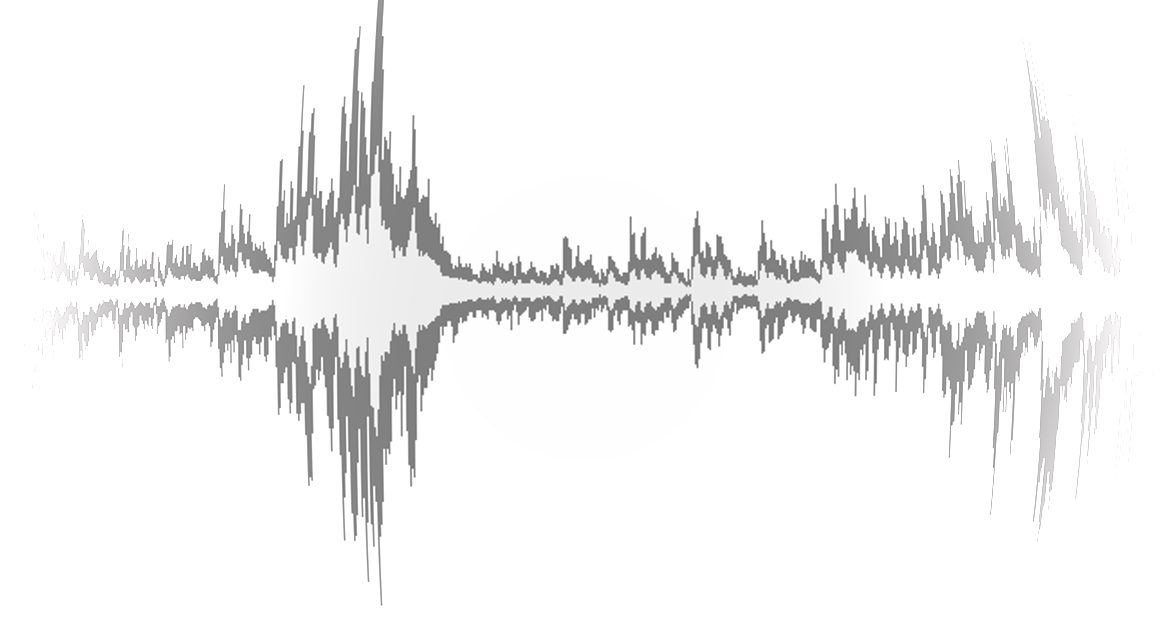
\includegraphics[width=\textwidth,height=3cm]{title}}

%%%%%%%%%%%%%%%%%%%%%%%%%%%%%%%%%%%%%%%%%%%%%%%%%%%%%%%%%%%%%%%%%%%%%%%%%%%%%%%%%%
%%%%%%%%%%%%%%%%%%%%%%%%%%%%%%%%%%%%%%%%%%%%%%%%%%%%%%%%%%%%%%%%%%%%%%%%%%%%%%%%%%
% colors
\definecolor{gtgold}{rgb}{.914, .664, 0} %0e7eed {rgb}{0.88,0.66,1,0.06} [234, 170, 0]/256 %96caff
\definecolor{darkgray}{rgb}{.15, .15, .15}
\definecolor{lightblue}{HTML}{0e7eed}
\definecolor{highlight}{rgb}{0, 0, 1} %_less!40

%%%%%%%%%%%%%%%%%%%%%%%%%%%%%%%%%%%%%%%%%%%%%%%%%%%%%%%%%%%%%%%%%%%%%%%%%%%%%%%%%%
%%%%%%%%%%%%%%%%%%%%%%%%%%%%%%%%%%%%%%%%%%%%%%%%%%%%%%%%%%%%%%%%%%%%%%%%%%%%%%%%%%
% relative paths
\graphicspath{{../graph/}}


%%%%%%%%%%%%%%%%%%%%%%%%%%%%%%%%%%%%%%%%%%%%%%%%%%%%%%%%%%%%%%%%%%%%%%%%%%%%%%%%%%
%%%%%%%%%%%%%%%%%%%%%%%%%%%%%%%%%%%%%%%%%%%%%%%%%%%%%%%%%%%%%%%%%%%%%%%%%%%%%%%%%%
% units
\setlength{\unitlength}{1mm}

%%%%%%%%%%%%%%%%%%%%%%%%%%%%%%%%%%%%%%%%%%%%%%%%%%%%%%%%%%%%%%%%%%%%%%%%%%%%%%%%%%
%%%%%%%%%%%%%%%%%%%%%%%%%%%%%%%%%%%%%%%%%%%%%%%%%%%%%%%%%%%%%%%%%%%%%%%%%%%%%%%%%%
% math
\DeclareMathOperator*{\argmax}{argmax}
\DeclareMathOperator*{\argmin}{argmin}
\DeclareMathOperator*{\atan}{atan}
\DeclareMathOperator*{\arcsinh}{arcsinh}
\DeclareMathOperator*{\sign}{sign}
\DeclareMathOperator*{\tcdf}{tcdf}
\DeclareMathOperator*{\si}{sinc}
\DeclareMathOperator*{\princarg}{princarg}
\DeclareMathOperator*{\arccosh}{arccosh}
\DeclareMathOperator*{\hwr}{HWR}
\DeclareMathOperator*{\flip}{flip}
\DeclareMathOperator*{\sinc}{sinc}
\DeclareMathOperator*{\floor}{floor}
\newcommand{\e}{{e}}
\newcommand{\jom}{\mathrm{j}\omega}
\newcommand{\jOm}{\mathrm{j}\Omega}
\newcommand   {\mat}[1]    		{\boldsymbol{\uppercase{#1}}}		%bold
\renewcommand {\vec}[1]    		{\boldsymbol{\lowercase{#1}}}		%bold

%%%%%%%%%%%%%%%%%%%%%%%%%%%%%%%%%%%%%%%%%%%%%%%%%%%%%%%%%%%%%%%%%%%%%%%%%%%%%%%%%%
%%%%%%%%%%%%%%%%%%%%%%%%%%%%%%%%%%%%%%%%%%%%%%%%%%%%%%%%%%%%%%%%%%%%%%%%%%%%%%%%%%
% media9
\newcommand{\includeaudio}[1]{
\href{run:audio/#1.mp3}{
\includegraphics[width=5mm, height=5mm]{graph/SpeakerIcon}}}

\newcommand{\includeanimation}[4]{{\begin{center}
                        \animategraphics[autoplay,loop,scale=.7]{#4}{animation/#1-}{#2}{#3}        
                        \end{center}
                        \addreference{matlab source: \href{https://github.com/alexanderlerch/ACA-Plots/blob/master/matlab/animate#1.m}{matlab/animate#1.m}}}
                        \inserticon{video}}
                        
%%%%%%%%%%%%%%%%%%%%%%%%%%%%%%%%%%%%%%%%%%%%%%%%%%%%%%%%%%%%%%%%%%%%%%%%%%%%%%%%%%
%%%%%%%%%%%%%%%%%%%%%%%%%%%%%%%%%%%%%%%%%%%%%%%%%%%%%%%%%%%%%%%%%%%%%%%%%%%%%%%%%%
% other commands
\newcommand{\question}[1]{%\vspace{-4mm}
                          \setbeamercovered{invisible}
                          \begin{columns}[T]
                            \column{.9\textwidth}
                                \textbf{#1}
                            \column{.1\textwidth}
                                \vspace{-8mm}
                                \begin{flushright}
                                     
\includegraphics[width=.9\columnwidth]{graph/question_mark}
                                \end{flushright}
                                \vspace{6mm}
                          \end{columns}\pause\vspace{-12mm}}

\newcommand{\toremember}[1]{
                        \inserticon{lightbulb}
                        }

\newcommand{\matlabexercise}[1]{%\vspace{-4mm}
                          \setbeamercovered{invisible}
                          \begin{columns}[T]
                            \column{.8\textwidth}
                                \textbf{matlab exercise}: #1
                            \column{.2\textwidth}
                                \begin{flushright}
                                     \includegraphics[scale=.5]{graph/logo_matlab}
                                \end{flushright}
                                %\vspace{6mm}
                          \end{columns}}

\newcommand{\addreference}[1]{  
                  
                    \begin{textblock*}{\baselineskip }(.98\paperwidth,.5\textheight) %(1.15\textwidth,.4\textheight)
                         \begin{minipage}[b][.5\paperheight][b]{1cm}%
                            \vfill%
                             \rotatebox{90}{\tiny {#1}}
                        \end{minipage}
                   \end{textblock*}
                    }
                    
\newcommand{\figwithmatlab}[1]{
                    \begin{figure}
                        \centering
                        \includegraphics[scale=.7]{#1}
                        %\label{fig:#1}
                    \end{figure}
                    
                    \addreference{matlab source: \href{https://github.com/alexanderlerch/MUSI-6202/blob/main/matlab/plot#1.m}{plot#1.m}}}
\newcommand{\figwithref}[2]{
                    \begin{figure}
                        \centering
                        \includegraphics[scale=.7]{#1}
                        \label{fig:#1}
                    \end{figure}
                    
                    \addreference{#2}}  
                                    
\newcommand{\inserticon}[1]{
                    \begin{textblock*}{100mm}(14.5cm,7.5cm)
                        \includegraphics[height=.8cm,keepaspectratio]{graph/#1}
                    \end{textblock*}}            

%%%%%%%%%%%%%%%%%%%%%%%%%%%%%%%%%%%%%%%%%%%%%%%%%%%%%%%%%%%%%%%%%%%%%%%%%%%%%%%%%%
%%%%%%%%%%%%%%%%%%%%%%%%%%%%%%%%%%%%%%%%%%%%%%%%%%%%%%%%%%%%%%%%%%%%%%%%%%%%%%%%%%
% counters
\newcounter{i}
\newcounter{j}
\newcounter{iXOffset}
\newcounter{iYOffset}
\newcounter{iXBlockSize}
\newcounter{iYBlockSize}
\newcounter{iYBlockSizeDiv2}
\newcounter{iXBlockSizeDiv2}
\newcounter{iDistance}

\newcommand{\IEEELink}{https://ieeexplore.ieee.org/servlet/opac?bknumber=9965970}

\addbibresource{../shared/references}



\subtitle{Part 23: Source Coding}

%%%%%%%%%%%%%%%%%%%%%%%%%%%%%%%%%%%%%%%%%%%%%%%%%%%%%%%%%%%%%%%%%%%%%%%%%%%%
\begin{document}
    % generate title page
	\title[]{Digital Signal Processing for Music}   
\author[alexander lerch]{alexander lerch} 
%\institute{~}
%\date[Alexander Lerch]{}
\titlegraphic{\vspace{-16mm}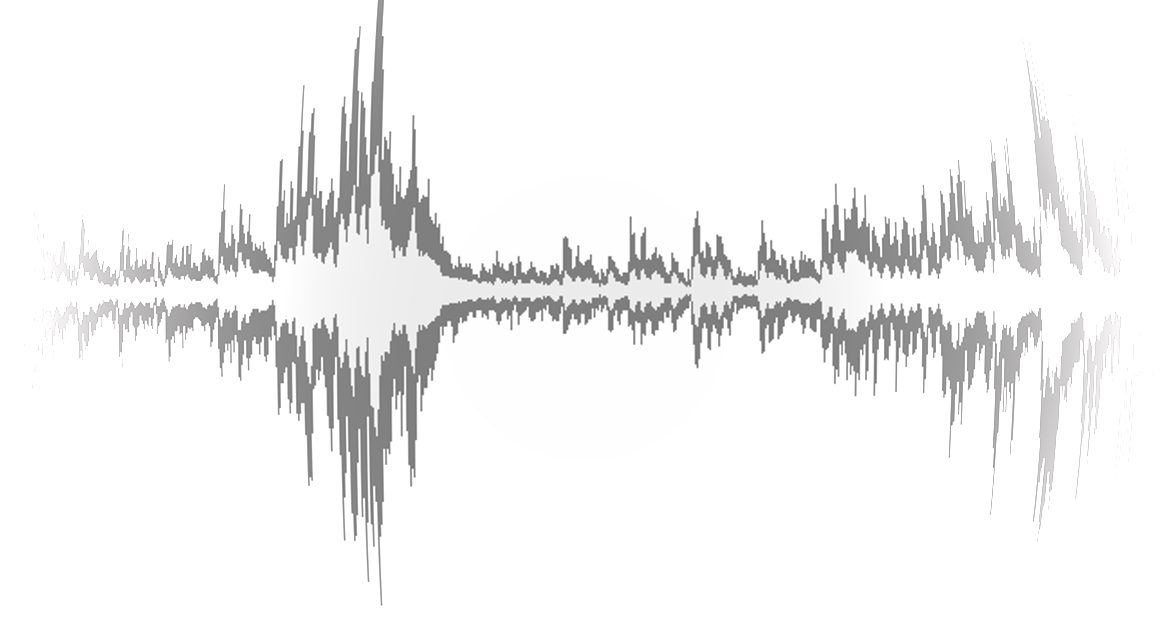
\includegraphics[width=\textwidth,height=3cm]{title}}


\begin{frame}
    \titlepage
    %\vspace{-5mm}
    \begin{flushright}
        \href{http://www.gtcmt.gatech.edu}{
\includegraphics[height=.8cm,keepaspectratio]{../shared/Logo_GTCMT_black}}
    \end{flushright}
\end{frame}


\section[intro]{introduction}

	\begin{frame}{source coding}{introduction 1/3}
		\begin{itemize}
			\item	typical audio \textbf{bit rates}
				\begin{eqnarray}
					\unit[16]{bit}\cdot\unit[44100]{sps}\cdot\unit[2]{chan} &=& \unit[1411.2]{kbps}\nonumber\\
					\unit[24]{bit}\cdot\unit[192000]{sps}\cdot\unit[5]{chan} &=& \unit[23040]{kbps}\nonumber
				\end{eqnarray}
			\vspace{-5mm}
			\item<2->	\textbf{reasons} for bit rate reduction
				\begin{itemize}
					\item	economical reasons: cheaper transmission/storage
					\item	technical reasons: restricted storage/transmission bandwidth
				\end{itemize}
			\smallskip
			\item<3->	\textbf{applications} for source coding
				\begin{itemize}
					\item	Internet: streaming, distribution, peer-2-peer, VoIP, \ldots
					\item	Media: DVD-V/A, \ldots
					\item	Portable Devices: MP3-Player, cell phones, Mini-Disc, \ldots
					\item	Broadcasting: (Digital) Radio, TV, \ldots
					\item	Cinema: DD, DTS, SDDS
					\item	\ldots
				\end{itemize}
		\end{itemize}
	\end{frame}
	\begin{frame}{source coding}{introduction 2/3}
        \question{How can the bitrate be reduced}
			
		\begin{enumerate}
			\item	\textbf{lossless}:\\ remove \textit{redundant} information (unnecessary to reconstruct the signal)
				\begin{itemize}
					\item	entropy coding
					\item	(linear predictive coding)
				\end{itemize}
			\pause
            \bigskip
			\item	\textbf{lossy}:\\ remove \textit{irrelevant} information (not ``missed'' by the recipient)
				\begin{itemize}
					\item	waveform coding
					\item	perceptual coding
				\end{itemize}
		\end{enumerate}
        \setbeamercovered{transparent}
	\end{frame}
	\begin{frame}{source coding}{introduction 3/3}
			\begin{figure}
				\centering
                \begin{picture}(50,50)
                    \put(0,25){\vector(1,0){50}}
                    \put(45,27){\footnotesize{\shortstack[c]{redundant}}}
                    
                    \put(25,0){\vector(0,1){50}}
                    \put(21,51){\footnotesize{\shortstack[c]{irrelevant}}}
                    
                    \put(0,0){\grid(25,25)(1.25,1.25)}
                    \put(5,10){\colorbox{white}{\framebox(15,8){\footnotesize{\shortstack[c]{\color{gtgold}{of interest}}}}}}
                 \end{picture}
					%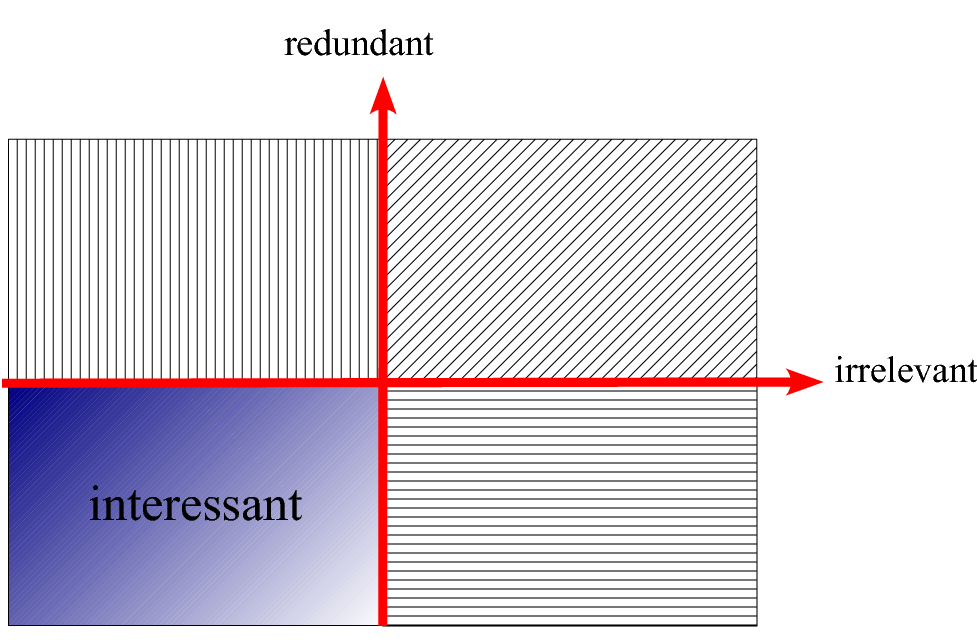
\includegraphics[scale=.3]{graph/redundancy_irrelevancy}
			\end{figure}
	\end{frame}
\section{information theory}
	\begin{frame}{source coding}{fundamentals: definitions}
		note: words to be transmitted are referred to as \textit{symbols}
		\pause
		\begin{block}{\textbf{information content}}
			\begin{columns}
            \column{.6\linewidth}
			The less frequent a symbol, the higher its \textit{information content}, \textit{self-information}, \textit{surprisal}.
            \column{.3\linewidth}
			\begin{equation*}
				I_n = \log_2\left(\frac{1}{p_n} \right)
			\end{equation*}
            \end{columns}
		\end{block}
		\pause
        \bigskip
		\begin{block}{\textbf{entropy}}
			\begin{columns}
            \column{.6\linewidth}
			The entropy is the \textit{Expected Value} of the information content. It is the \textit{theoretic minimum of bits} required for transmission.
            \column{.3\linewidth}
			\begin{equation*}
				H = \sum\limits_{n=0}^{N-1}{p_n\cdot I_n}
			\end{equation*}
            \end{columns}
			
		\end{block}
	\end{frame}

	\begin{frame}{source coding}{fundamentals: information content and entropy examples}
        \setbeamercovered{invisible}
		\begin{itemize}
			\item	\textbf{dice}: $p_n = \frac{1}{6}$
			\begin{eqnarray*}
				I_n &=& \log_2\left(\frac{1}{p_n}\right)  = 2.58\; bit\\
				H &=& 6 \cdot \frac{1}{6} \cdot 2.58\; bit % \unit[2.58]{bit}
			\end{eqnarray*}
			\pause
			\item	\textbf{imperfect dice}: $p_1 = \frac{1}{2},\; p_{2\ldots 6} = \frac{1}{10}$
			\pause
			\begin{eqnarray*}
				I_1 &=  \log_2\left(2\right)  &= 1\; bit \\
				I_{2\ldots 6} &= \log_2\left(10\right)  &= 3.32\; bit \\
				H &= \frac{1}{2}\cdot 1 + \frac{5}{10}\cdot 3.32 &= 2.16\; bit %\unit[2.16]{bit}
			\end{eqnarray*}
		\end{itemize}
        \setbeamercovered{transparent}
	\end{frame}

\section{entropy coding}
	\begin{frame}{source coding}{entropy coding: example 1}
		\textbf{idea: use shorter words for frequent symbols}
		\pause
		\begin{itemize}
			\item	3 possible symbols
			\begin{table}
				\begin{center}
				\begin{footnotesize}
					\begin{tabular}{lccc}
					\hline
						\textbf{symbol}  & \textbf{probability} & \textbf{word}\\
					\hline
					A & $p=0.5$	& \only<3->{$0$}\\
					B & $p=0.25$	& \only<3->{$10$}\\
					C & $p=0.25$	& \only<3->{$11$}\\
					\end{tabular}  
				\end{footnotesize}
				\end{center}
			\end{table}
			\pause
			\item	entropy
			\begin{equation*}
				H = \sum\limits_{n=0}^{N-1}{p_n\log_2\left(\frac{1}{p_n} \right)} = 1.5
			\end{equation*}
			\pause
			\item	transmit the following group of symbols: $ABCA\rightarrow \; 010110$
			
			\pause
			\item required bits:
			\begin{equation*}
				\frac{transmitted \; bits}{transmitted\; symbols} = \frac{6}{4} = 1.5
			\end{equation*}
			\pause
			$\Rightarrow$ \color{gtgold}{optimal transmission}
		\end{itemize}
	\end{frame}

	\begin{frame}{source coding}{entropy coding: example 2}
		\begin{itemize}
		
			\item 3 possible symbols
			\begin{table}
				\begin{center}
				\begin{footnotesize}
					\begin{tabular}{lccc}
					\hline
						\textbf{symbol} & \textbf{probability} & \textbf{word} \\
					\hline
					A &	 $p=0.7$	& \only<2->{$0$}\\
					B &	$p=0.2$	& \only<2->{$10$}\\
					C &	$p=0.1$	& \only<2->{$11$}\\
					\end{tabular}  
				\end{footnotesize}
				\end{center}
			\end{table}
			\pause
			\item	entropy
			\begin{equation*}
				H = \sum\limits_{n=0}^N{p_n\log_2\left(\frac{1}{p_n} \right)} = 1.11
			\end{equation*}
			\pause
			\item	transmit the following group of symbols: $ABCA\rightarrow \; 010110$

			\pause
			\item required bits:
			\begin{equation*}
				\frac{transmitted \; bits}{transmitted\; symbols} = \frac{6}{4} = 1.5
			\end{equation*}
			\pause
			$\Rightarrow$ \color{gtgold}{\textit{non}-optimal transmission}
		\end{itemize}
	\end{frame}
	
	\begin{frame}{source coding}{huffman coding: tree construction 1/2}
        \vspace{-4mm}
			\begin{table}
				\begin{center}
				\begin{footnotesize}
					\begin{tabular}{lc}
						\parbox{50mm}{sort symbols acc.\ to frequency} & 
						\begin{tabular}{cc}
							frequency & symbol\\
							5	& 1\\
							7	& 2\\
							10	& 3\\
							15	& 4\\
							20	& 5\\
							45	& 6
						\end{tabular}\\

						\parbox{50mm}{combine two lowest symbols into new entry (sum)} & 
						\begin{picture}(15,12)
							\put(6, 8){\text{12:*}}
							\put(0, 0){\text{5:1}}
							\put(13, 0){\text{7:2}}
							\put(14, 4){\line(-1,1){3}}
							\put(2, 4){\line(1,1){3}}
						\end{picture}\\
						\parbox{50mm}{add new entry to list} & 
						\begin{tabular}{cc}
							frequency & symbol\\
							10	& 3\\
							12	& *\\
							15	& 4\\
							20	& 5\\
							45	& 6
						\end{tabular}\\
						\parbox{50mm}{repeat until only one element left in the list} & 
					\end{tabular}  
				\end{footnotesize}
				\end{center}
			\end{table}
	\end{frame}
	\begin{frame}{source coding}{huffman coding: tree construction 2/2}
    \vspace{-5mm}
    \begin{columns}
    \column{.7\linewidth}
	\begin{center}
	\begin{picture}(70, 50)
		\only<1-2>{
			\put(0, 47){\only<2>{\textcolor{gtgold}}{\text{5:1}}}
			\put(13, 47){\only<2>{\textcolor{gtgold}}{\text{7:2}}}
			\put(26, 47){\text{10:3}}
			\put(39, 47){\text{15:4}}
			\put(52, 47){\text{20:5}}
			\put(65, 47){\text{45:6}}
		}
		\only<3-4>{
			\put(13, 47){\only<4>{\textcolor{gtgold}}{\text{10:3}}}
			\put(26, 47){\only<4>{\textcolor{gtgold}}{\text{12:*}}}
			\put(39, 47){\text{15:4}}
			\put(52, 47){\text{20:5}}
			\put(65, 47){\text{45:6}}
			
				\put(20, 39){\text{5:1}}
				\put(33, 39){\text{7:2}}
				\put(23, 43){\line(1,1){3}}
				\put(34, 43){\line(-1,1){3}}
			
		}
		\only<5-6>{
			\put(13, 47){\only<6>{\textcolor{gtgold}}{\text{15:4}}}
			\put(26, 47){\only<6>{\textcolor{gtgold}}{\text{20:5}}}
			\put(39, 47){\text{22:*}}
			\put(65, 47){\text{45:6}}
			
				\put(33, 39){\text{10:3}}
				\put(46, 39){\text{12:*}}
				\put(36, 43){\line(1,1){3}}
				\put(47, 43){\line(-1,1){3}}

					\put(40, 31){\text{5:1}}
					\put(53, 31){\text{7:2}}
					\put(43, 35){\line(1,1){3}}
					\put(54, 35){\line(-1,1){3}}
			
		}
		\only<7-8>{
			\put(26, 47){\only<8>{\textcolor{gtgold}}{\text{22:*}}}
			\put(52, 47){\only<8>{\textcolor{gtgold}}{\text{35:*}}}
			\put(65, 47){\text{45:6}}

				\put(20, 39){\text{10:3}}
				\put(33, 39){\text{12:*}}
				\put(23, 43){\line(1,1){3}}
				\put(34, 43){\line(-1,1){3}}
			
				\put(46, 39){\text{15:4}}
				\put(59, 39){\text{20:5}}
				\put(49, 43){\line(1,1){3}}
				\put(60, 43){\line(-1,1){3}}

					\put(27, 31){\text{5:1}}
					\put(40, 31){\text{7:2}}
					\put(30, 35){\line(1,1){3}}
					\put(41, 35){\line(-1,1){3}}
			
		}
		\only<9-10>{
			\put(13, 47){\only<10>{\textcolor{gtgold}}{\text{45:6}}}
			\put(39, 47){\only<10>{\textcolor{gtgold}}{\text{57:*}}}

				\put(26, 39){\text{22:*}}
				\put(52, 39){\text{35:*}}
				\put(29, 43){\line(1,1){3}}
				\put(53, 43){\line(-1,1){3}}

					\put(20, 31){\text{10:3}}
					\put(33, 31){\text{12:*}}
					\put(23, 35){\line(1,1){3}}
					\put(34, 35){\line(-1,1){3}}
				
					\put(46, 31){\text{15:4}}
					\put(59, 31){\text{20:5}}
					\put(49, 35){\line(1,1){3}}
					\put(60, 35){\line(-1,1){3}}
	
						\put(27, 23){\text{5:1}}
						\put(40, 23){\text{7:2}}
						\put(30, 27){\line(1,1){3}}
						\put(41, 27){\line(-1,1){3}}
		}
		\only<11->{
			\put(26, 47){\text{102:*}}

				\put(13, 39){\text{45:6}}
				\put(39, 39){\text{57:*}}
				\put(16, 43){\line(1,1){3}}
				\put(40, 43){\line(-1,1){3}}
	
					\put(26, 31){\text{22:*}}
					\put(52, 31){\text{35:*}}
					\put(29, 35){\line(1,1){3}}
					\put(53, 35){\line(-1,1){3}}
	
						\put(20, 23){\text{10:3}}
						\put(33, 23){\text{12:*}}
						\put(23, 27){\line(1,1){3}}
						\put(34, 27){\line(-1,1){3}}
					
						\put(46, 23){\text{15:4}}
						\put(59, 23){\text{20:5}}
						\put(49, 27){\line(1,1){3}}
						\put(60, 27){\line(-1,1){3}}
		
							\put(27, 15){\text{5:1}}
							\put(40, 15){\text{7:2}}
							\put(30, 19){\line(1,1){3}}
							\put(41, 19){\line(-1,1){3}}
		}
		\only<12->{
			\put(14, 44){\textcolor{gtgold}{\text{\textbf{0}}}}
			\put(27, 36){\textcolor{gtgold}{\text{\textbf{0}}}}
			\put(21, 28){\textcolor{gtgold}{\text{\textbf{0}}}}
			\put(47, 28){\textcolor{gtgold}{\text{\textbf{0}}}}
			\put(28, 20){\textcolor{gtgold}{\text{\textbf{0}}}}

			\put(41, 44){\textcolor{gtgold}{\text{\textbf{1}}}}
			\put(53, 36){\textcolor{gtgold}{\text{\textbf{1}}}}
			\put(34, 28){\textcolor{gtgold}{\text{\textbf{1}}}}
			\put(60, 28){\textcolor{gtgold}{\text{\textbf{1}}}}
			\put(41, 20){\textcolor{gtgold}{\text{\textbf{1}}}}
		}
	\end{picture}	
	\end{center}
    \column{.3\linewidth}
		\only<13->{
			%\vspace{-15mm}
			\begin{table}
				\begin{center}
					\begin{footnotesize}
						\begin{tabular}{ccc}
							\textbf{frequency} & \textbf{symbol} & \textbf{code}\\
							5	& 1 & 1010\\
							7	& 2 & 1011\\
							10	& 3 & 100\\
							15	& 4 & 110\\
							20	& 5 & 111\\
							45	& 6 & 0
						\end{tabular}
					\end{footnotesize}
				\end{center}
			\end{table}
		}
	\end{columns}
        \only<14->{
			\begin{itemize}
				\item[note:]	no code is prefix of another code!
			\end{itemize}
            }
	\end{frame}
	
	\begin{frame}{source coding}{huffman coding for audio signals}
		\begin{itemize}
			\item	Symbole: $2^w$
			\pause
			\item	PDF indicates probability per symbol
				\figwithmatlab{Rfd}
		\end{itemize}
	\end{frame}
	
	\begin{frame}{source coding}{arithmetic coding}
		\begin{itemize}
			\item	\textbf{Huffman coding is only optimal if $p_n = \frac{1}{2^k}$}
			\pause
            \bigskip
			\item	alternative: \textbf{arithmetic coding} 
                \begin{itemize}
                    \item   allows other probability distributions
                    \item   encodes the whole sequence in one fractional number $0.0 \leq f < 1.0$
                    \pause
                    \bigskip
                    \item   \textbf{principle}: 
                        \begin{enumerate}
                            \item   assume initial interval of $[0,1[$ 
                            \pause
                            \item   assign interval segments to all symbols, e.g. $A = [0,0.7[, B= [0.7,0.9[, C=[0.9,1[$
                            \pause
                            \item   select interval based on current symbol
                            \pause
                            \item	go to Step 2. or terminate
                        \end{enumerate}
                \end{itemize}
				%\begin{enumerate}
					%\item	set the initial interval to $[0,1[$
					%\item	split the interval into regions corresponding to probabilities, e.g. $A = [0,0.7], B= [0.7,0.9[, C=[0.9,1[$
					%\item	choose the new interval to be that of the current symbol
					%\item	go to Step 2.
					%\item	terminate with special symbol
				%\end{enumerate}	
		\end{itemize}
	\end{frame}
	
	\begin{frame}{source coding}{arithmetic coding: example 1/2}
            \vspace{-3mm}
                \begin{footnotesize}
            sequence $ABCA$, $p_\mathrm{A} = 0.6, p_\mathrm{B}= 0.2, p_\mathrm{C}=0.1, p_\mathrm{T}=0.1$, \pause\mbox{\footnotesize $A = [0,0.6[, B= [0.6,0.8[, C=[0.8,0.9[, T=[0.9,1[$}
        %\begin{columns}
            %\column{.1\linewidth}
            %\column{.9\linewidth}
            %\pause
				\begin{itemize}
					\item	\textbf{decoding} 0.463: 
                        \begin{enumerate}
							\item	$0.463 \in$ segment 1 ($\rightarrow A$), 
                                \begin{itemize}
                                    \item set interval $[0,0.6[$ $ \rightarrow$ {bounds: $0,0.36,0.48,0.54,0.6$}
                                \end{itemize}
							\pause
                            \item	$0.463 \in$ segment 2 ($\rightarrow B$),
                                \begin{itemize}
                                    \item set interval $[0.36,0.48[$ $ \rightarrow$ {bounds: } {\footnotesize $0.36,0.432,0.456,0.468,0.48$}
                                \end{itemize}
							\pause
                            \item	$0.463 \in$ segment 3 ($\rightarrow C$), 
                                \begin{itemize}
                                    \item set interval $[0.456,0.468[$ $ \rightarrow$ {bounds: } {\footnotesize $0.456,0.4632,0.4656,0.4668,0.468$}
                                \end{itemize}
							\pause
                            \item	$0.463 \in$ segment 1 ($\rightarrow A$), 
                                \begin{itemize}
                                    \item set interval $[0.456, 0.4632[$ $ \rightarrow$ {bounds: } {\footnotesize $0.456,0.46032,0.46176,0.46248,0.4632$}
                                \end{itemize}
							\pause
                            \item   $0.463 \in$ segment 4 ($\rightarrow$ terminate)
						\end{enumerate}
		\end{itemize}
                \end{footnotesize}
	\end{frame}
	
	\begin{frame}{source coding}{arithmetic coding: example 2/2}
            \vspace{-3mm}
                \begin{footnotesize}
            sequence $ABCA$, $p_\mathrm{A} = 0.6, p_\mathrm{B}= 0.2, p_\mathrm{C}=0.1, p_\mathrm{T}=0.1$, \pause\mbox{\footnotesize $A = [0,0.6[, B= [0.6,0.8[, C=[0.8,0.9[, T=[0.9,1[$}
        %\begin{columns}
            %\column{.1\linewidth}
            %\column{.9\linewidth}
            %\pause
				\begin{itemize}
					\item \textbf{encoding} 
						\begin{enumerate}
							\item	select segment 1, set interval to $[0,0.6[$
							\pause
							\item	select segment 2, set interval to $[0.36,0.48[$
							\pause
							\item	select segment 3, set interval to $[0.456,0.468[$
							\pause
							\item	select segment 1, set interval to $[0.456, 0.4632[$
							\pause
                            \item   select segment 4, set interval to $[0.46248, 0.4632[$
							\pause
							\item   choose value from last segment (e.g., 0.463) and transmit
						\end{enumerate}
				\end{itemize}
                \end{footnotesize}
        %\end{columns}
	\end{frame}
		
\section{linear prediction}
	\begin{frame}{source coding}{fundamentals: linear prediction}
		idea: use preceding samples to estimate/predict future samples.
		\begin{itemize}
			\item	\textbf{estimate the signal} x
				\begin{equation*}
					\hat{x}(i) = \sum\limits_{j=1}^{\mathcal{O}}{b_j\cdot x(i-j)}
				\end{equation*}
			\pause
			\item	prediction quality is measured by \textbf{power of prediction error}
				\begin{eqnarray*}
					e_{\mathrm{P}}(i)	&=& x(i)-\hat{x}(i)\\
							&=& x(i) - \sum\limits_{j=1}^{\mathcal{O}}{b_j\cdot x(i-j)}
				\end{eqnarray*}
		\end{itemize}						
	\end{frame}
	\begin{frame}{source coding}{fundamentals: linear prediction --- first order prediction 1/2}
        \vspace{-4mm}
        \begin{itemize}
            \item   \textbf{prediction}
                $\hat{x}(i) = b_1\cdot x(i-1)$
            \item<2->   \textbf{prediction error}
                \begin{footnotesize}
				\begin{eqnarray*}
                    \sigma_e^2 &=& \mathcal{E}\left\lbrace (x(i)-b_1x(i-1))^2\right\rbrace\\
                    &=& \sigma_x^2 + b_1^2 \sigma_x^2 -2b_1 r_{xx}(1)\\
                    &=& \left(1 + b_1^2 - 2b_1\rho_{xx}(1)\right) \sigma_x^2
				\end{eqnarray*}
                \end{footnotesize}
            \item<3->   \textbf{optimum coefficient}: $\frac{\partial\sigma_e^2}{\partial b_1} = 0$
                \begin{footnotesize}
				\begin{eqnarray*}
                    2b_1\sigma_x^2 - 2\rho_{xx}(1)\sigma_x^2 &=& 0\\
                    b_1 &=& \rho_{xx}(1)
				\end{eqnarray*}
                \end{footnotesize}
                \vspace{-4mm}
            \item<4->   \textbf{minimum prediction error power}
                \begin{footnotesize}
				\begin{eqnarray*}
                    \sigma_e^2 &=& \left(1 + b_1^2 - 2b_1\rho_{xx}(1)\right) \sigma_x^2\\
                    &=& \left(1 + \rho_{xx}(1)^2 - 2\rho_{xx}(1)\rho_{xx}(1)\right) \sigma_x^2\\
                    &=& (1-\rho_{xx}(1))\sigma_x^2
				\end{eqnarray*}
                \end{footnotesize}
        \end{itemize}
	\end{frame}
	\begin{frame}{source coding}{fundamentals: linear prediction --- first order prediction 2/2}
        \begin{equation*}
            \sigma_e^2 = (1-\rho_{xx}(1))\sigma_x^2
        \end{equation*}
        
        \begin{itemize}
            \item             \textbf{observations}:
            \begin{itemize}
                \item   power of prediction error always smaller or equal the power of the signal
                \item   question: when is it equal to the signal?
            \end{itemize}
            \bigskip
            \item<2->   \textbf{special case}: $b_1 = 1$
                \begin{eqnarray*}
                    \hat{x}(i) &=& x(i-1)\\
                    e_\mathrm{P} &=& x(i) - x(i-1)\\
                    \sigma_e^2 &=& (1 + b_1^2 -2b_1\rho_{xx}(1))\sigma_x^2\\
                    &=& 2(1-\rho_{xx}(1))\sigma_x^2
                \end{eqnarray*}
        \end{itemize}
	\end{frame}
	\begin{frame}{source coding}{fundamentals: linear prediction --- prediction coefficients}
        \vspace{-3mm}
		\begin{itemize}
			\item	prediction gain depends on
				\begin{itemize}
					\item	predictor coefficients $b_j$
					\item	signal
				\end{itemize}
			\pause
            \bigskip
			\item	optimal coefficients can be derived by finding minimum of prediction error
				\begin{equation*}
					\frac{\partial \sigma_e^2}{\partial b_j} = 0
				\end{equation*}
				$\Rightarrow$ (without derivation)
			\begin{equation*}
				r_{xx}(\eta) = \sum\limits_{j=1}^{\mathcal{O}}{b_{j,\mathrm{opt}}\cdot r_{xx}(\eta-j)} ,\;\;\;\;\; 1 \leq\eta\leq\mathcal{O} 
			\end{equation*}	
            \begin{eqnarray*}
                \vec{r}_{xx} &=& \mat{R}_{xx}\cdot \vec{b}_\mathrm{opt}\\
                \vec{b}_\mathrm{opt} &=& \mat{R}_{xx}^{-1}\cdot \vec{r}_{xx}
            \end{eqnarray*}
		\end{itemize}						
	\end{frame}
	\begin{frame}{source coding}{fundamentals: linear prediction --- summary}
		\begin{itemize}
			\item 	\textbf{predictor length}
				\begin{itemize}
					\item	rule of thumb: the longer the predictor, the better the prediction
					\item	can range from 10 coefficients to hundreds
				\end{itemize}
			\pause
            \bigskip
			\item	\textbf{predictor coefficient updates}
				\begin{itemize}
					\item	better signal adaptation if coefficients are updated block-by-block
				\end{itemize}
			\pause
            \bigskip
			\item	\textbf{input signals}
				\begin{itemize}
					\item	white noise/random processes cannot be predicted
					\item	periodic signals may theoretically be perfectly predicted
				\end{itemize}
		\end{itemize}
	\end{frame}
	\begin{frame}{source coding}{fundamentals: linear prediction --- audio example}
        order: 20
        \begin{columns}
            \column{.7\textwidth}
            \figwithmatlab{LinPred}
%%			\begin{figure}
%%				\centering
					%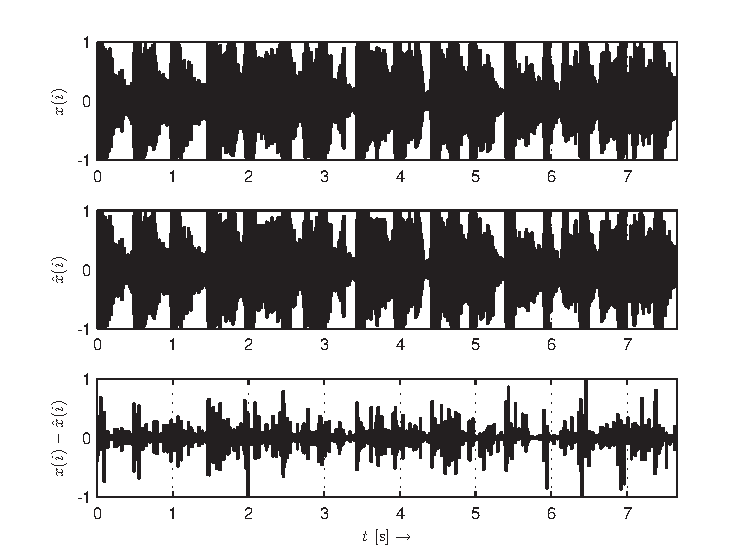
\includegraphics[scale=0.6]{graph/linearprediction}
%%			\end{figure}
			\column{.3\textwidth}
                \vspace{6mm}
                
                \includeaudio{jamo_snippet}
                
                \vspace{8mm}

                \includeaudio{jamo_snippet_Pred}
                
                \vspace{8mm}

                \includeaudio{jamo_snippet_PredError}
			\end{columns}
	\end{frame}

\section{joint channels}
	\begin{frame}{source coding}{fundamentals: joint channels}
        \vspace{-3mm}
        \begin{columns}
            \column{.8\textwidth}
				\figwithmatlab{MS}
			\column{.3\textwidth}
                %\vspace{6mm}
                
                \includeaudio{jamo_snippet}
                
                \vspace{19mm}
                
                \includeaudio{jamo_snippet_M}
                $M = \frac{L+R}{2}$
                
                \vspace{4mm}
                
                \includeaudio{jamo_snippet_S}
                $S = \frac{R-L}{2}$
			\end{columns}
			\vspace{-5mm}
            \begin{eqnarray*}
                L &=& M + S\\
                R &=& M - S 
            \end{eqnarray*}
	\end{frame}

	
	
\section{summary}
		\begin{frame}{source coding}{summary}
            \begin{itemize}
                \item   bitrate can be reduced by removing removing redundancy and/or irrelevance
                \smallskip
                \item   removing redundancy:
                    \begin{itemize}
                        \item   entropy coding: transmit frequent symbols with shorter codes
                        \item   linear prediction: transmit diff signal plus predictor coefficients
                    \end{itemize}
                \smallskip
                \item   removing irrelevance:
                    \begin{itemize}
                        \item   reduce quantization wordlength
                        \item   see slides below
                    \end{itemize}
            \end{itemize}
 		\end{frame}

\end{document}

